\documentclass[twoside]{book}

% Packages required by doxygen
\usepackage{fixltx2e}
\usepackage{calc}
\usepackage{doxygen}
\usepackage[export]{adjustbox} % also loads graphicx
\usepackage{graphicx}
\usepackage[utf8]{inputenc}
\usepackage{makeidx}
\usepackage{multicol}
\usepackage{multirow}
\PassOptionsToPackage{warn}{textcomp}
\usepackage{textcomp}
\usepackage[nointegrals]{wasysym}
\usepackage[table]{xcolor}

% Font selection
\usepackage[T1]{fontenc}
\usepackage[scaled=.90]{helvet}
\usepackage{courier}
\usepackage{amssymb}
\usepackage{sectsty}
\renewcommand{\familydefault}{\sfdefault}
\allsectionsfont{%
  \fontseries{bc}\selectfont%
  \color{darkgray}%
}
\renewcommand{\DoxyLabelFont}{%
  \fontseries{bc}\selectfont%
  \color{darkgray}%
}
\newcommand{\+}{\discretionary{\mbox{\scriptsize$\hookleftarrow$}}{}{}}

% Page & text layout
\usepackage{geometry}
\geometry{%
  a4paper,%
  top=2.5cm,%
  bottom=2.5cm,%
  left=2.5cm,%
  right=2.5cm%
}
\tolerance=750
\hfuzz=15pt
\hbadness=750
\setlength{\emergencystretch}{15pt}
\setlength{\parindent}{0cm}
\setlength{\parskip}{3ex plus 2ex minus 2ex}
\makeatletter
\renewcommand{\paragraph}{%
  \@startsection{paragraph}{4}{0ex}{-1.0ex}{1.0ex}{%
    \normalfont\normalsize\bfseries\SS@parafont%
  }%
}
\renewcommand{\subparagraph}{%
  \@startsection{subparagraph}{5}{0ex}{-1.0ex}{1.0ex}{%
    \normalfont\normalsize\bfseries\SS@subparafont%
  }%
}
\makeatother

% Headers & footers
\usepackage{fancyhdr}
\pagestyle{fancyplain}
\fancyhead[LE]{\fancyplain{}{\bfseries\thepage}}
\fancyhead[CE]{\fancyplain{}{}}
\fancyhead[RE]{\fancyplain{}{\bfseries\leftmark}}
\fancyhead[LO]{\fancyplain{}{\bfseries\rightmark}}
\fancyhead[CO]{\fancyplain{}{}}
\fancyhead[RO]{\fancyplain{}{\bfseries\thepage}}
\fancyfoot[LE]{\fancyplain{}{}}
\fancyfoot[CE]{\fancyplain{}{}}
\fancyfoot[RE]{\fancyplain{}{\bfseries\scriptsize Generated by Doxygen }}
\fancyfoot[LO]{\fancyplain{}{\bfseries\scriptsize Generated by Doxygen }}
\fancyfoot[CO]{\fancyplain{}{}}
\fancyfoot[RO]{\fancyplain{}{}}
\renewcommand{\footrulewidth}{0.4pt}
\renewcommand{\chaptermark}[1]{%
  \markboth{#1}{}%
}
\renewcommand{\sectionmark}[1]{%
  \markright{\thesection\ #1}%
}

% Indices & bibliography
\usepackage{natbib}
\usepackage[titles]{tocloft}
\setcounter{tocdepth}{3}
\setcounter{secnumdepth}{5}
\makeindex

% Hyperlinks (required, but should be loaded last)
\usepackage{ifpdf}
\ifpdf
  \usepackage[pdftex,pagebackref=true]{hyperref}
\else
  \usepackage[ps2pdf,pagebackref=true]{hyperref}
\fi
\hypersetup{%
  colorlinks=true,%
  linkcolor=blue,%
  citecolor=blue,%
  unicode%
}

% Custom commands
\newcommand{\clearemptydoublepage}{%
  \newpage{\pagestyle{empty}\cleardoublepage}%
}

\usepackage{caption}
\captionsetup{labelsep=space,justification=centering,font={bf},singlelinecheck=off,skip=4pt,position=top}

%===== C O N T E N T S =====

\begin{document}

% Titlepage & ToC
\hypersetup{pageanchor=false,
             bookmarksnumbered=true,
             pdfencoding=unicode
            }
\pagenumbering{roman}
\begin{titlepage}
\vspace*{7cm}
\begin{center}%
{\Large Erriez J\+Y-\/\+L\+K\+M1638 board library for Arduino \\[1ex]\large 1.\+1.\+0 }\\
\vspace*{1cm}
{\large Generated by Doxygen 1.8.11}\\
\end{center}
\end{titlepage}
\clearemptydoublepage
\tableofcontents
\clearemptydoublepage
\pagenumbering{arabic}
\hypersetup{pageanchor=true}

%--- Begin generated contents ---
\chapter{J\+Y-\/\+L\+K\+M1638 7-\/segment display / button library for Arduino}
\label{index}\hypertarget{index}{}This is a J\+Y-\/\+M\+CU J\+Y-\/\+L\+K\+M1638 library for Arduino.



This board supports\+:
\begin{DoxyItemize}
\item 3-\/wire serial interface
\item T\+M1638 L\+ED driver and key-\/scan chip
\item Power\+: 3.\+3V .. 5V
\item 8 digits 7-\/segment display
\item 8 dual color L\+E\+Ds
\item 8 buttons
\end{DoxyItemize}

\subsection*{Order number}

\href{https://www.google.nl/search?q=JY-LKM1638}{\tt Google.\+com} \href{http://www.dx.com/p/8x-digital-tube-8x-key-8x-double-color-led-module-81873#.WmR3YTco9aR}{\tt D\+X.\+com S\+K\+U\+: 81873} \href{https://www.aliexpress.com/item/F71A-8-Digital-Tube-8-Key-8-Double-Color-LED-Module-TM1638-Can-be-Cascaded-Replace/2034831073.html?ws_ab_test=searchweb0_0,searchweb201602_1_10065_10344_10068_10342_10343_10340_10341_10084_10083_10618_10304_10615_10307_10301_10313_10059_10534_100031_10103_441_10624_442_10623_10622_10621_10620_10142,searchweb201603_36,ppcSwitch_5&algo_expid=539835e4-fcbf-4f84-870e-c972d12374fa-36&algo_pvid=539835e4-fcbf-4f84-870e-c972d12374fa&priceBeautifyAB=2}{\tt Ali\+Express.\+com} \href{https://www.ebay.com/itm/8xDigital-Tube-8x-Key-8x-Double-Color-LED-Module-TM1638-For-AVR-Arduino-NEW/172744309516?epid=814196876&hash=item28385cfb0c:g:bmsAAOSw-29ZS4-c}{\tt e\+Bay.\+com} Many more...

{\bfseries Note\+:} This library has not been tested with a different \char`\"{}\+L\+E\+D\&\+K\+E\+Y\char`\"{} board.

\subsection*{Hardware}

Connect G\+ND and +5V to the Arduino board.

Connect the following pins to the Arduino D\+I\+G\+I\+T\+AL pins\+:
\begin{DoxyItemize}
\item D\+IO (Bi-\/directional data input/output)
\item S\+TB (Chip select)
\item C\+LK (Clock)
\end{DoxyItemize}

Note\+: Some Arduino boards cannot deliver enough 5V power to drive the L\+ED\textquotesingle{}s.

\subsubsection*{Pins}

\tabulinesep=1mm
\begin{longtabu} spread 0pt [c]{*5{|X[-1]}|}
\hline
\rowcolor{\tableheadbgcolor}\PBS\centering {\bf Pin }&\PBS\centering {\bf L\+K\+M-\/1638 }&\PBS\centering {\bf Arduino U\+NO / Nano / Mega2560 / Leonardo / Pro Micro }&\PBS\centering {\bf Node M\+CU }&\PBS\centering {\bf L\+O\+L\+I\+N32  }\\\cline{1-5}
\endfirsthead
\hline
\endfoot
\hline
\rowcolor{\tableheadbgcolor}\PBS\centering {\bf Pin }&\PBS\centering {\bf L\+K\+M-\/1638 }&\PBS\centering {\bf Arduino U\+NO / Nano / Mega2560 / Leonardo / Pro Micro }&\PBS\centering {\bf Node M\+CU }&\PBS\centering {\bf L\+O\+L\+I\+N32  }\\\cline{1-5}
\endhead
\PBS\centering 1 &\PBS\centering V\+CC &\PBS\centering 5V (or 3.\+3V) &\PBS\centering G\+ND &\PBS\centering G\+ND \\\cline{1-5}
\PBS\centering 2 &\PBS\centering G\+ND &\PBS\centering G\+ND &\PBS\centering 3\+V3 &\PBS\centering 3\+V3 \\\cline{1-5}
\PBS\centering 3 &\PBS\centering C\+LK &\PBS\centering Digital pin 2 &\PBS\centering D2 &\PBS\centering 0 \\\cline{1-5}
\PBS\centering 4 &\PBS\centering D\+IO &\PBS\centering Digital pin 3 &\PBS\centering D3 &\PBS\centering 4 \\\cline{1-5}
\PBS\centering 5 &\PBS\centering S\+T\+B1 &\PBS\centering Digital pin 4 &\PBS\centering D4 &\PBS\centering 5 \\\cline{1-5}
\end{longtabu}


\subsection*{Examples}

Examples $\vert$ J\+Y-\/\+L\+K\+M1638\+:
\begin{DoxyItemize}
\item \href{https://github.com/Erriez/ErriezLKM1638/blob/master/examples/Brightness/Brightness.ino}{\tt Brightness}
\item \href{https://github.com/Erriez/ErriezLKM1638/blob/master/examples/Buttons/Buttons.ino}{\tt Buttons}
\item \href{https://github.com/Erriez/ErriezLKM1638/blob/master/examples/Counter/Counter.ino}{\tt Counter}
\item \href{https://github.com/Erriez/ErriezLKM1638/blob/master/examples/Date/Date.ino}{\tt Date}
\item \href{https://github.com/Erriez/ErriezLKM1638/blob/master/examples/Demo/Demo.ino}{\tt Demo}
\item \href{https://github.com/Erriez/ErriezLKM1638/blob/master/examples/Temperature/Temperature.ino}{\tt Temperature}
\item \href{https://github.com/Erriez/ErriezLKM1638/blob/master/examples/TestLEDs/TestLEDs.ino}{\tt Test\+L\+E\+Ds}
\item \href{https://github.com/Erriez/ErriezLKM1638/blob/master/examples/Time/Time.ino}{\tt Time}
\end{DoxyItemize}

\subsection*{Documentation}


\begin{DoxyItemize}
\item \href{https://erriez.github.io/ErriezLKM1638}{\tt Doxygen online H\+T\+ML}
\item \href{https://github.com/Erriez/ErriezLKM1638/raw/gh-pages/latex/ErriezLKM1638.pdf}{\tt Doxygen P\+DF}
\end{DoxyItemize}

\#\# Terms\+: 
\begin{DoxyCode}
1 Segment:   One LED in a 7-segment display
2 Digit:     One 7-segment display (Value 0..9 and A..F)
3 Dot:       The dot LED in a 7-segment digit
4 Pos:       Print position 0...7 (MSB bit 7: left .. LB bit 0: right)
5 Radius:    DEC for decimal, HEX for hexadecimal, BIN for binary
6 MaxDigits: Reserve a number of digits to print a value
7 Pad:       Display fixed number of digits with 0 padding
8 Overflow:  Value does not fit on the display, display minus chars
9 LSB:       Most right digit, dual color LED8 or switch (SW8)
10 MSB:       Most left digit,  dual color LED1 or switch (SW1)
\end{DoxyCode}


\subsection*{Usage}

\#\#\# Initialization 
\begin{DoxyCode}
1 \{c++\}
2 #include <LKM1638Board.h>
3 
4 // Connect display pins to the Arduino DIGITAL pins
5 #define TM1638\_CLK\_PIN   2
6 #define TM1638\_DIO\_PIN   3
7 #define TM1638\_STB0\_PIN  4
8 
9 // Create LKM1638 board
10 LKM1638Board lkm1638(TM1638\_CLK\_PIN, TM1638\_DIO\_PIN, TM1638\_STB0\_PIN);
11 
12 void setup()
13 \{
14     // Initialize LKM1638Board
15     lkm1638.begin();
16 \}
\end{DoxyCode}


\subsubsection*{Read 8 buttons}

Buttons are 8-\/bit with bit 7 most left switch, bit 0 most right switch.

Note\+: The text on the board counts from S1 to S8!


\begin{DoxyCode}
1 \{c++\}
2 uint8\_t buttons = lkm1638.getButtons();
\end{DoxyCode}


\subsubsection*{Control 8 dual color L\+ED\textquotesingle{}s}

Dual color L\+ED 7 = most left (Text L\+E\+D8) Dual color L\+ED 0 = most right (Text L\+E\+D0)


\begin{DoxyCode}
1 \{c++\}
2 // Turn LED 0 red on (firt LED on the right)
3 lkm1638.setColorLED(0, LedRed);  
4 
5 // Turn LED 0 green on
6 lkm1638.setColorLED(0, LedGreen);
7 
8 // Turn LED 0 off
9 lkm1638.setColorLED(0, LedOff);
10 
11 // Turn multiple LEDs on, color red
12 lkm1638.colorLEDsOn(0xA9, LedRed);
13 
14 // Turn multiple LEDs off
15 lkm1638.colorLEDsOff(0x1F);
\end{DoxyCode}


\#\#\# Clear display 
\begin{DoxyCode}
1 \{c++\}
2 lkm1638.clear();
\end{DoxyCode}


\subsubsection*{Set/get print display position}

The print position can be set from 0..7. 7 = most left digit 0 = most right digit


\begin{DoxyCode}
1 \{c++\}
2 // Set postion 4
3 lkm1638.setPrintPos(4);
4 
5 // Get print position
6 uint8\_t pos = lkm1638.getPrintPos();
\end{DoxyCode}


\subsubsection*{Print variable on 7-\/segment display}

Printing starts from digit right to left with an optional maximum number of digits.

Minus \textquotesingle{}-\/\textquotesingle{} chars will be displayed when the value is out of range, or does not fit on the display.

Optional padding can be used to display zero\textquotesingle{}s. This is for example useful to print hours and minutes with fixed 2 digits.


\begin{DoxyCode}
1 \{c++\}
2 // Print int16\_t on print position
3 lkm1638.print(1234);
4 
5 // Print signed 32-bit value
6 lkm1638.print(-1234567);
7 
8 // Print 16-bit unsigned casted value
9 lkm1638.print((uint16\_t)65535);
10 
11 // Print 16-bit hexadecimal unsigned value
12 uint16\_t value = 0xBEEF;
13 lkm1638.print(value, HEX); 
14 
15 // Print value with maximum 2 digits
16 uint8\_t value = 99;
17 lkm1638.print(value++, DEC, 2);
18 
19 // Print -- when value is greater than 2 digits 
20 lkm1638.print(value, DEC, 2); 
21 
22 // Print 16-bit unsigned value with max 4 digits and 4 digits padding: 0009 
23 uint16\_t value = 9;
24 lkm1638.print(value, DEC, 4, 4);
25 
26 // Print 32-bit unsigned value
27 lkm1638.print(12345678UL);
28 
29 // Print binary uint8\_t 0xA9 = 10101001
30 uint8\_t value = 0xA9;
31 lkm1638.print(value, BIN, 8, 8);
\end{DoxyCode}


\#\#\# Control 8 display dots 
\begin{DoxyCode}
1 \{c++\}
2 // Turn one dot on in digit 7 (most left)
3 lkm1638.dotOn(7);
4 
5 // Turn one dot off in digit 0 (most right)
6 lkm1638.dotOff(0);
7 
8 // Set multiple dots on and off
9 lkm1638.setDots(0x85);
\end{DoxyCode}


\#\#\# Display special characters 
\begin{DoxyCode}
1 \{c++\}
2 // Turn digit off
3 lkm1638.setSegmentsDigit(5, SEGMENTS\_OFF);
4 
5 // Display minus character
6 lkm1638.setSegmentsDigit(4, SEGMENTS\_MINUS);
7 
8 // Display degree selsius symbol + C
9 lkm1638.setSegmentsDigit(1, SEGMENTS\_DEGREE);
10 lkm1638.setSegmentsDigit(0, SEGMENTS\_C);
\end{DoxyCode}


\#\#\# Write a custom character to the display 
\begin{DoxyCode}
1 \{c++\}
2 // Display single LED in a digit
3 lkm1638.setSegmentsDigit(0, 0b0001000);
\end{DoxyCode}


\subsection*{Library dependencies}


\begin{DoxyItemize}
\item \href{https://github.com/Erriez/ErriezTM1638}{\tt Erriez T\+M1638}
\end{DoxyItemize}

\subsection*{Library installation}

Please refer to the \href{https://github.com/Erriez/ErriezArduinoLibrariesAndSketches/wiki}{\tt Wiki} page.

\subsection*{Other Arduino Libraries and Sketches from Erriez}


\begin{DoxyItemize}
\item \href{https://github.com/Erriez/ErriezArduinoLibrariesAndSketches}{\tt Erriez Libraries and Sketches} 
\end{DoxyItemize}
\chapter{Hierarchical Index}
\section{Class Hierarchy}
This inheritance list is sorted roughly, but not completely, alphabetically\+:\begin{DoxyCompactList}
\item T\+M1638\begin{DoxyCompactList}
\item \contentsline{section}{L\+K\+M1638\+Board}{\pageref{class_l_k_m1638_board}}{}
\end{DoxyCompactList}
\end{DoxyCompactList}

\chapter{Class Index}
\section{Class List}
Here are the classes, structs, unions and interfaces with brief descriptions\+:\begin{DoxyCompactList}
\item\contentsline{section}{\hyperlink{class_l_k_m1638_board}{L\+K\+M1638\+Board} \\*\hyperlink{class_l_k_m1638_board}{L\+K\+M1638\+Board} class, derived from T\+M1638 library }{\pageref{class_l_k_m1638_board}}{}
\end{DoxyCompactList}

\chapter{File Index}
\section{File List}
Here is a list of all documented files with brief descriptions\+:\begin{DoxyCompactList}
\item\contentsline{section}{\hyperlink{_l_k_m1638_board_8cpp}{L\+K\+M1638\+Board.\+cpp} \\*J\+Y-\/\+L\+K\+M1638 board v1.\+1 library for Arduino }{\pageref{_l_k_m1638_board_8cpp}}{}
\item\contentsline{section}{\hyperlink{_l_k_m1638_board_8h}{L\+K\+M1638\+Board.\+h} \\*J\+Y-\/\+L\+K\+M1638 board v1.\+1 library for Arduino }{\pageref{_l_k_m1638_board_8h}}{}
\end{DoxyCompactList}

\chapter{Class Documentation}
\hypertarget{class_l_k_m1638_board}{}\section{L\+K\+M1638\+Board Class Reference}
\label{class_l_k_m1638_board}\index{L\+K\+M1638\+Board@{L\+K\+M1638\+Board}}


\hyperlink{class_l_k_m1638_board}{L\+K\+M1638\+Board} class, derived from T\+M1638 library.  




{\ttfamily \#include $<$L\+K\+M1638\+Board.\+h$>$}

Inheritance diagram for L\+K\+M1638\+Board\+:\begin{figure}[H]
\begin{center}
\leavevmode
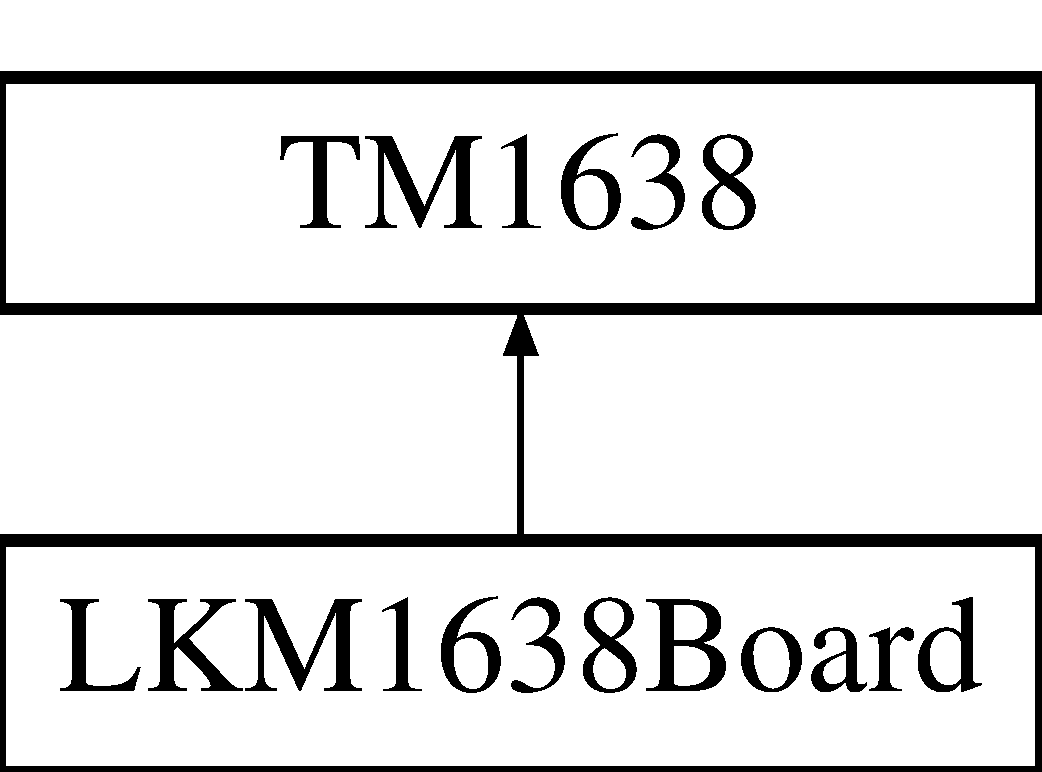
\includegraphics[height=2.000000cm]{class_l_k_m1638_board}
\end{center}
\end{figure}
\subsection*{Public Member Functions}
\begin{DoxyCompactItemize}
\item 
\hyperlink{class_l_k_m1638_board_a8526eb1bc413de3ea12c78b79d5d4bef}{L\+K\+M1638\+Board} (uint8\+\_\+t clk\+Pin, uint8\+\_\+t dio\+Pin, uint8\+\_\+t stb\+Pin)
\begin{DoxyCompactList}\small\item\em L\+K\+M1638 constructor. \end{DoxyCompactList}\item 
uint8\+\_\+t \hyperlink{class_l_k_m1638_board_a46b3777daa6d86b5a0e871fb99604898}{get\+Buttons} ()
\begin{DoxyCompactList}\small\item\em Read buttons. \end{DoxyCompactList}\item 
void \hyperlink{class_l_k_m1638_board_a487398df6c28769e87f20ea51e1395ee}{clear} ()\hypertarget{class_l_k_m1638_board_a487398df6c28769e87f20ea51e1395ee}{}\label{class_l_k_m1638_board_a487398df6c28769e87f20ea51e1395ee}

\begin{DoxyCompactList}\small\item\em Turn all L\+ED\textquotesingle{}s off. \end{DoxyCompactList}\item 
void \hyperlink{class_l_k_m1638_board_a58ee1bc95f31491e1e3d1bd67a85ca07}{set\+Color\+L\+ED} (uint8\+\_\+t led, \hyperlink{_l_k_m1638_board_8h_a81ea3de5b76240d46410f8b9acf4cbde}{Led\+Color} color)
\begin{DoxyCompactList}\small\item\em Set dual color L\+ED. \end{DoxyCompactList}\item 
void \hyperlink{class_l_k_m1638_board_a9c563169a60f4010b89449dce438ccb7}{color\+L\+E\+Ds\+On} (uint8\+\_\+t leds, \hyperlink{_l_k_m1638_board_8h_a81ea3de5b76240d46410f8b9acf4cbde}{Led\+Color} color)
\begin{DoxyCompactList}\small\item\em Turn multiple color L\+ED\textquotesingle{}s on. \end{DoxyCompactList}\item 
void \hyperlink{class_l_k_m1638_board_abf401ad1fa384a03732ed6e6d558ba2b}{color\+L\+E\+Ds\+Off} (uint8\+\_\+t leds)
\begin{DoxyCompactList}\small\item\em Turn multiple color L\+ED\textquotesingle{}s off. \end{DoxyCompactList}\item 
void \hyperlink{class_l_k_m1638_board_affcd16cf2844a7596f08251fab8e0d40}{refresh} ()\hypertarget{class_l_k_m1638_board_affcd16cf2844a7596f08251fab8e0d40}{}\label{class_l_k_m1638_board_affcd16cf2844a7596f08251fab8e0d40}

\begin{DoxyCompactList}\small\item\em Refresh display. \end{DoxyCompactList}\item 
void \hyperlink{class_l_k_m1638_board_adf22c1b3001db91ed263bd5952b2ea5c}{dot\+On} (uint8\+\_\+t pos)
\begin{DoxyCompactList}\small\item\em Turn dot L\+ED on. \end{DoxyCompactList}\item 
void \hyperlink{class_l_k_m1638_board_ad946f70d7cabf87562fd3482e010462b}{dot\+Off} (uint8\+\_\+t pos)
\begin{DoxyCompactList}\small\item\em Turn dot L\+ED off. \end{DoxyCompactList}\item 
void \hyperlink{class_l_k_m1638_board_a50f9693ca74fef320fb3898cdf4480c4}{set\+Dots} (uint8\+\_\+t dots)
\begin{DoxyCompactList}\small\item\em Turn multiple dots on or off. \end{DoxyCompactList}\item 
void \hyperlink{class_l_k_m1638_board_a6d91010acd57d05179a3d6c2435993f3}{set\+Print\+Pos} (uint8\+\_\+t pos)
\begin{DoxyCompactList}\small\item\em Set print position. \end{DoxyCompactList}\item 
uint8\+\_\+t \hyperlink{class_l_k_m1638_board_ad50f047120592ae1c70de9528475d0f7}{get\+Print\+Pos} ()
\begin{DoxyCompactList}\small\item\em Get print position. \end{DoxyCompactList}\item 
void \hyperlink{class_l_k_m1638_board_afd4d21ac6046c65eac7198e831d959ad}{set\+Segments\+Digit} (uint8\+\_\+t pos, uint8\+\_\+t leds)
\begin{DoxyCompactList}\small\item\em Write L\+ED segments of a digit. \end{DoxyCompactList}\item 
void \hyperlink{class_l_k_m1638_board_a8776f66e796c3ea9e389ea6aa50dcef2}{set\+Digit} (uint8\+\_\+t pos, uint8\+\_\+t digit)
\begin{DoxyCompactList}\small\item\em Write digit. \end{DoxyCompactList}\item 
void \hyperlink{class_l_k_m1638_board_a02dedfb608775b702d17e4d993006bec}{print} (uint8\+\_\+t value)
\begin{DoxyCompactList}\small\item\em Print uint8\+\_\+t value. \end{DoxyCompactList}\item 
void \hyperlink{class_l_k_m1638_board_a4c2dfa4e41c625419af04b23f67d55c0}{print} (uint8\+\_\+t value, uint8\+\_\+t radius)
\begin{DoxyCompactList}\small\item\em Print uint8\+\_\+t with radius. \end{DoxyCompactList}\item 
void \hyperlink{class_l_k_m1638_board_a162d7463e2a5a61c8d2688a0ccc2469f}{print} (uint8\+\_\+t value, uint8\+\_\+t radius, uint8\+\_\+t max\+Digits)
\begin{DoxyCompactList}\small\item\em Print uint8\+\_\+t with radius and maximum number of digits. \end{DoxyCompactList}\item 
void \hyperlink{class_l_k_m1638_board_ae38bc4ef7ce51c10adbf0a4708ee9f8d}{print} (uint8\+\_\+t value, uint8\+\_\+t radius, uint8\+\_\+t max\+Digits, uint8\+\_\+t pad)
\begin{DoxyCompactList}\small\item\em Print uint8\+\_\+t with radius, maximum number of digits and padding digits. \end{DoxyCompactList}\item 
void {\bfseries print} (uint16\+\_\+t value)\hypertarget{class_l_k_m1638_board_addb92b7db50eae92e3e5a493b2254e32}{}\label{class_l_k_m1638_board_addb92b7db50eae92e3e5a493b2254e32}

\item 
void {\bfseries print} (uint16\+\_\+t value, uint8\+\_\+t radius)\hypertarget{class_l_k_m1638_board_aa23737222e7b89c3788a0b989d875c8e}{}\label{class_l_k_m1638_board_aa23737222e7b89c3788a0b989d875c8e}

\item 
void {\bfseries print} (uint16\+\_\+t value, uint8\+\_\+t radius, uint8\+\_\+t max\+Digits)\hypertarget{class_l_k_m1638_board_a00a327012ce4139379fd7db2b9c18d46}{}\label{class_l_k_m1638_board_a00a327012ce4139379fd7db2b9c18d46}

\item 
void {\bfseries print} (uint16\+\_\+t value, uint8\+\_\+t radius, uint8\+\_\+t max\+Digits, uint8\+\_\+t pad)\hypertarget{class_l_k_m1638_board_ada91bebab1bbf9a0b49c2badbc719a23}{}\label{class_l_k_m1638_board_ada91bebab1bbf9a0b49c2badbc719a23}

\item 
void {\bfseries print} (unsigned long value)\hypertarget{class_l_k_m1638_board_a7bcc87b42a36593c0dc25f96d35dd7b7}{}\label{class_l_k_m1638_board_a7bcc87b42a36593c0dc25f96d35dd7b7}

\item 
void {\bfseries print} (unsigned long value, uint8\+\_\+t radius)\hypertarget{class_l_k_m1638_board_a3ad79f70f43abe6cdd93e0820451ee2e}{}\label{class_l_k_m1638_board_a3ad79f70f43abe6cdd93e0820451ee2e}

\item 
void {\bfseries print} (unsigned long value, uint8\+\_\+t radius, uint8\+\_\+t max\+Digits)\hypertarget{class_l_k_m1638_board_a58d41caae5893ba5de7d0f0b1694e603}{}\label{class_l_k_m1638_board_a58d41caae5893ba5de7d0f0b1694e603}

\item 
void {\bfseries print} (unsigned long value, uint8\+\_\+t radius, uint8\+\_\+t max\+Digits, uint8\+\_\+t pad)\hypertarget{class_l_k_m1638_board_a4d85c9a6d46429371f53d48d88bcf098}{}\label{class_l_k_m1638_board_a4d85c9a6d46429371f53d48d88bcf098}

\item 
void {\bfseries print} (int8\+\_\+t value)\hypertarget{class_l_k_m1638_board_a3870dd214f2cf1f8fef72914caf6514f}{}\label{class_l_k_m1638_board_a3870dd214f2cf1f8fef72914caf6514f}

\item 
void {\bfseries print} (int8\+\_\+t value, uint8\+\_\+t radius)\hypertarget{class_l_k_m1638_board_a3ef6e7753b0bb41fce28beb6929ff322}{}\label{class_l_k_m1638_board_a3ef6e7753b0bb41fce28beb6929ff322}

\item 
void {\bfseries print} (int8\+\_\+t value, uint8\+\_\+t radius, uint8\+\_\+t max\+Digits)\hypertarget{class_l_k_m1638_board_a45e0efcafa18905ffbe54418c5bd9882}{}\label{class_l_k_m1638_board_a45e0efcafa18905ffbe54418c5bd9882}

\item 
void {\bfseries print} (int16\+\_\+t value)\hypertarget{class_l_k_m1638_board_a6a528db7d882c863343ebc3113121144}{}\label{class_l_k_m1638_board_a6a528db7d882c863343ebc3113121144}

\item 
void {\bfseries print} (int16\+\_\+t value, uint8\+\_\+t radius)\hypertarget{class_l_k_m1638_board_a4319c529f3c73460d711b9a1a4be7ca0}{}\label{class_l_k_m1638_board_a4319c529f3c73460d711b9a1a4be7ca0}

\item 
void {\bfseries print} (int16\+\_\+t value, uint8\+\_\+t radius, uint8\+\_\+t max\+Digits)\hypertarget{class_l_k_m1638_board_aa272bb1dbb3efa68775183dce20900eb}{}\label{class_l_k_m1638_board_aa272bb1dbb3efa68775183dce20900eb}

\item 
void {\bfseries print} (long value)\hypertarget{class_l_k_m1638_board_a15473b5559176286ee1f91e157725c55}{}\label{class_l_k_m1638_board_a15473b5559176286ee1f91e157725c55}

\item 
void {\bfseries print} (long value, uint8\+\_\+t radius)\hypertarget{class_l_k_m1638_board_abd76f4879932dcafed65972c2ccefddb}{}\label{class_l_k_m1638_board_abd76f4879932dcafed65972c2ccefddb}

\item 
void {\bfseries print} (long value, uint8\+\_\+t radius, uint8\+\_\+t max\+Digits)\hypertarget{class_l_k_m1638_board_acf4c5b99e65c269e9871ac1cf96b2c24}{}\label{class_l_k_m1638_board_acf4c5b99e65c269e9871ac1cf96b2c24}

\end{DoxyCompactItemize}
\subsection*{Protected Member Functions}
\begin{DoxyCompactItemize}
\item 
void \hyperlink{class_l_k_m1638_board_a186ecd4a644171428fbd93aa7f309ccb}{write\+Digit} (uint8\+\_\+t pos)
\begin{DoxyCompactList}\small\item\em Write digit position. \end{DoxyCompactList}\item 
void \hyperlink{class_l_k_m1638_board_a54932b39bb7571604299d1c25d334086}{write\+Unsigned\+Value} (uint32\+\_\+t value, uint8\+\_\+t radius, uint8\+\_\+t max\+Digits, uint8\+\_\+t pad)
\begin{DoxyCompactList}\small\item\em Write unsigned value to display. \end{DoxyCompactList}\item 
void \hyperlink{class_l_k_m1638_board_acacc4f02b25f985486f625af9e6edce5}{write\+Signed\+Value} (int32\+\_\+t value, uint8\+\_\+t radius, uint8\+\_\+t max\+Digits)
\begin{DoxyCompactList}\small\item\em Write signed value to display. \end{DoxyCompactList}\item 
uint8\+\_\+t \hyperlink{class_l_k_m1638_board_ad56606fb7bca18eb6a3f16d45a8d294b}{get\+Num\+Digits} (uint32\+\_\+t value, uint8\+\_\+t radius)
\begin{DoxyCompactList}\small\item\em Get number of digits of a signed 32-\/bit value. \end{DoxyCompactList}\item 
void \hyperlink{class_l_k_m1638_board_abaffb270a3b1baa76d15416ff6c0aa30}{display\+Overflow} (uint8\+\_\+t num\+Digits)
\begin{DoxyCompactList}\small\item\em Display overflow with -\/ characters. \end{DoxyCompactList}\item 
uint8\+\_\+t \hyperlink{class_l_k_m1638_board_aef7255786ce884f881b84b6d182fbaad}{swap\+Bits} (uint8\+\_\+t data)
\begin{DoxyCompactList}\small\item\em Swap bits. \end{DoxyCompactList}\item 
uint8\+\_\+t \hyperlink{class_l_k_m1638_board_a36bc06324f7f4bb412d42338e4adfb18}{swap\+Pos} (uint8\+\_\+t pos)
\begin{DoxyCompactList}\small\item\em Swap digit position. \end{DoxyCompactList}\item 
uint8\+\_\+t \hyperlink{class_l_k_m1638_board_a9526953f337a0f5780c963f5e37a77d3}{swap\+Leds} (uint8\+\_\+t led)
\begin{DoxyCompactList}\small\item\em Swap dual color L\+ED\textquotesingle{}s. \end{DoxyCompactList}\end{DoxyCompactItemize}
\subsection*{Protected Attributes}
\begin{DoxyCompactItemize}
\item 
uint8\+\_\+t \hyperlink{class_l_k_m1638_board_ad0ecb25b0069693153b4c99b1fd0c0c6}{\+\_\+leds} \mbox{[}\hyperlink{_l_k_m1638_board_8h_a0b79fa1bdb1363440df485691386a74c}{N\+U\+M\+\_\+\+D\+I\+G\+I\+TS}\mbox{]}\hypertarget{class_l_k_m1638_board_ad0ecb25b0069693153b4c99b1fd0c0c6}{}\label{class_l_k_m1638_board_ad0ecb25b0069693153b4c99b1fd0c0c6}

\begin{DoxyCompactList}\small\item\em L\+ED digits. \end{DoxyCompactList}\item 
uint8\+\_\+t \hyperlink{class_l_k_m1638_board_a1dc0720aa961510a147cb7e3db7d7873}{\+\_\+pos}\hypertarget{class_l_k_m1638_board_a1dc0720aa961510a147cb7e3db7d7873}{}\label{class_l_k_m1638_board_a1dc0720aa961510a147cb7e3db7d7873}

\begin{DoxyCompactList}\small\item\em Print position. \end{DoxyCompactList}\item 
uint8\+\_\+t \hyperlink{class_l_k_m1638_board_a2de77cd6c33672edb5a3288b09cdcbfc}{\+\_\+dots}\hypertarget{class_l_k_m1638_board_a2de77cd6c33672edb5a3288b09cdcbfc}{}\label{class_l_k_m1638_board_a2de77cd6c33672edb5a3288b09cdcbfc}

\begin{DoxyCompactList}\small\item\em Dot L\+ED\textquotesingle{}s. \end{DoxyCompactList}\end{DoxyCompactItemize}


\subsection{Detailed Description}
\hyperlink{class_l_k_m1638_board}{L\+K\+M1638\+Board} class, derived from T\+M1638 library. 

Definition at line 66 of file L\+K\+M1638\+Board.\+h.



\subsection{Constructor \& Destructor Documentation}
\index{L\+K\+M1638\+Board@{L\+K\+M1638\+Board}!L\+K\+M1638\+Board@{L\+K\+M1638\+Board}}
\index{L\+K\+M1638\+Board@{L\+K\+M1638\+Board}!L\+K\+M1638\+Board@{L\+K\+M1638\+Board}}
\subsubsection[{\texorpdfstring{L\+K\+M1638\+Board(uint8\+\_\+t clk\+Pin, uint8\+\_\+t dio\+Pin, uint8\+\_\+t stb\+Pin)}{LKM1638Board(uint8_t clkPin, uint8_t dioPin, uint8_t stbPin)}}]{\setlength{\rightskip}{0pt plus 5cm}L\+K\+M1638\+Board\+::\+L\+K\+M1638\+Board (
\begin{DoxyParamCaption}
\item[{uint8\+\_\+t}]{clk\+Pin, }
\item[{uint8\+\_\+t}]{dio\+Pin, }
\item[{uint8\+\_\+t}]{stb\+Pin}
\end{DoxyParamCaption}
)}\hypertarget{class_l_k_m1638_board_a8526eb1bc413de3ea12c78b79d5d4bef}{}\label{class_l_k_m1638_board_a8526eb1bc413de3ea12c78b79d5d4bef}


L\+K\+M1638 constructor. 


\begin{DoxyParams}{Parameters}
{\em clk\+Pin} & Clock pin \\
\hline
{\em dio\+Pin} & Data pin (bi-\/directional) \\
\hline
{\em stb\+Pin} & Strobe pin (low is enable) \\
\hline
\end{DoxyParams}


Definition at line 80 of file L\+K\+M1638\+Board.\+cpp.



\subsection{Member Function Documentation}
\index{L\+K\+M1638\+Board@{L\+K\+M1638\+Board}!color\+L\+E\+Ds\+Off@{color\+L\+E\+Ds\+Off}}
\index{color\+L\+E\+Ds\+Off@{color\+L\+E\+Ds\+Off}!L\+K\+M1638\+Board@{L\+K\+M1638\+Board}}
\subsubsection[{\texorpdfstring{color\+L\+E\+Ds\+Off(uint8\+\_\+t leds)}{colorLEDsOff(uint8_t leds)}}]{\setlength{\rightskip}{0pt plus 5cm}void L\+K\+M1638\+Board\+::color\+L\+E\+Ds\+Off (
\begin{DoxyParamCaption}
\item[{uint8\+\_\+t}]{leds}
\end{DoxyParamCaption}
)}\hypertarget{class_l_k_m1638_board_abf401ad1fa384a03732ed6e6d558ba2b}{}\label{class_l_k_m1638_board_abf401ad1fa384a03732ed6e6d558ba2b}


Turn multiple color L\+ED\textquotesingle{}s off. 


\begin{DoxyParams}{Parameters}
{\em leds} & Byte with 8 L\+ED\textquotesingle{}s \\
\hline
\end{DoxyParams}


Definition at line 190 of file L\+K\+M1638\+Board.\+cpp.

\index{L\+K\+M1638\+Board@{L\+K\+M1638\+Board}!color\+L\+E\+Ds\+On@{color\+L\+E\+Ds\+On}}
\index{color\+L\+E\+Ds\+On@{color\+L\+E\+Ds\+On}!L\+K\+M1638\+Board@{L\+K\+M1638\+Board}}
\subsubsection[{\texorpdfstring{color\+L\+E\+Ds\+On(uint8\+\_\+t leds, Led\+Color color)}{colorLEDsOn(uint8_t leds, LedColor color)}}]{\setlength{\rightskip}{0pt plus 5cm}void L\+K\+M1638\+Board\+::color\+L\+E\+Ds\+On (
\begin{DoxyParamCaption}
\item[{uint8\+\_\+t}]{leds, }
\item[{{\bf Led\+Color}}]{color}
\end{DoxyParamCaption}
)}\hypertarget{class_l_k_m1638_board_a9c563169a60f4010b89449dce438ccb7}{}\label{class_l_k_m1638_board_a9c563169a60f4010b89449dce438ccb7}


Turn multiple color L\+ED\textquotesingle{}s on. 


\begin{DoxyParams}{Parameters}
{\em leds} & Byte with 8 L\+ED\textquotesingle{}s \\
\hline
{\em color} & 0\+: Off 1\+: Green 2\+: Red \\
\hline
\end{DoxyParams}


Definition at line 177 of file L\+K\+M1638\+Board.\+cpp.

\index{L\+K\+M1638\+Board@{L\+K\+M1638\+Board}!display\+Overflow@{display\+Overflow}}
\index{display\+Overflow@{display\+Overflow}!L\+K\+M1638\+Board@{L\+K\+M1638\+Board}}
\subsubsection[{\texorpdfstring{display\+Overflow(uint8\+\_\+t num\+Digits)}{displayOverflow(uint8_t numDigits)}}]{\setlength{\rightskip}{0pt plus 5cm}void L\+K\+M1638\+Board\+::display\+Overflow (
\begin{DoxyParamCaption}
\item[{uint8\+\_\+t}]{num\+Digits}
\end{DoxyParamCaption}
)\hspace{0.3cm}{\ttfamily [protected]}}\hypertarget{class_l_k_m1638_board_abaffb270a3b1baa76d15416ff6c0aa30}{}\label{class_l_k_m1638_board_abaffb270a3b1baa76d15416ff6c0aa30}


Display overflow with -\/ characters. 


\begin{DoxyParams}{Parameters}
{\em num\+Digits} & Number of digits to display \\
\hline
\end{DoxyParams}


Definition at line 575 of file L\+K\+M1638\+Board.\+cpp.

\index{L\+K\+M1638\+Board@{L\+K\+M1638\+Board}!dot\+Off@{dot\+Off}}
\index{dot\+Off@{dot\+Off}!L\+K\+M1638\+Board@{L\+K\+M1638\+Board}}
\subsubsection[{\texorpdfstring{dot\+Off(uint8\+\_\+t pos)}{dotOff(uint8_t pos)}}]{\setlength{\rightskip}{0pt plus 5cm}void L\+K\+M1638\+Board\+::dot\+Off (
\begin{DoxyParamCaption}
\item[{uint8\+\_\+t}]{pos}
\end{DoxyParamCaption}
)}\hypertarget{class_l_k_m1638_board_ad946f70d7cabf87562fd3482e010462b}{}\label{class_l_k_m1638_board_ad946f70d7cabf87562fd3482e010462b}


Turn dot L\+ED off. 


\begin{DoxyParams}{Parameters}
{\em pos} & Position 0..7 \\
\hline
\end{DoxyParams}


Definition at line 275 of file L\+K\+M1638\+Board.\+cpp.

\index{L\+K\+M1638\+Board@{L\+K\+M1638\+Board}!dot\+On@{dot\+On}}
\index{dot\+On@{dot\+On}!L\+K\+M1638\+Board@{L\+K\+M1638\+Board}}
\subsubsection[{\texorpdfstring{dot\+On(uint8\+\_\+t pos)}{dotOn(uint8_t pos)}}]{\setlength{\rightskip}{0pt plus 5cm}void L\+K\+M1638\+Board\+::dot\+On (
\begin{DoxyParamCaption}
\item[{uint8\+\_\+t}]{pos}
\end{DoxyParamCaption}
)}\hypertarget{class_l_k_m1638_board_adf22c1b3001db91ed263bd5952b2ea5c}{}\label{class_l_k_m1638_board_adf22c1b3001db91ed263bd5952b2ea5c}


Turn dot L\+ED on. 


\begin{DoxyParams}{Parameters}
{\em pos} & Position 0..7 \\
\hline
\end{DoxyParams}


Definition at line 263 of file L\+K\+M1638\+Board.\+cpp.

\index{L\+K\+M1638\+Board@{L\+K\+M1638\+Board}!get\+Buttons@{get\+Buttons}}
\index{get\+Buttons@{get\+Buttons}!L\+K\+M1638\+Board@{L\+K\+M1638\+Board}}
\subsubsection[{\texorpdfstring{get\+Buttons()}{getButtons()}}]{\setlength{\rightskip}{0pt plus 5cm}uint8\+\_\+t L\+K\+M1638\+Board\+::get\+Buttons (
\begin{DoxyParamCaption}
{}
\end{DoxyParamCaption}
)}\hypertarget{class_l_k_m1638_board_a46b3777daa6d86b5a0e871fb99604898}{}\label{class_l_k_m1638_board_a46b3777daa6d86b5a0e871fb99604898}


Read buttons. 

\begin{DoxyReturn}{Returns}
Value of 8 buttons 
\end{DoxyReturn}


Definition at line 93 of file L\+K\+M1638\+Board.\+cpp.

\index{L\+K\+M1638\+Board@{L\+K\+M1638\+Board}!get\+Num\+Digits@{get\+Num\+Digits}}
\index{get\+Num\+Digits@{get\+Num\+Digits}!L\+K\+M1638\+Board@{L\+K\+M1638\+Board}}
\subsubsection[{\texorpdfstring{get\+Num\+Digits(uint32\+\_\+t value, uint8\+\_\+t radius)}{getNumDigits(uint32_t value, uint8_t radius)}}]{\setlength{\rightskip}{0pt plus 5cm}uint8\+\_\+t L\+K\+M1638\+Board\+::get\+Num\+Digits (
\begin{DoxyParamCaption}
\item[{uint32\+\_\+t}]{value, }
\item[{uint8\+\_\+t}]{radius}
\end{DoxyParamCaption}
)\hspace{0.3cm}{\ttfamily [protected]}}\hypertarget{class_l_k_m1638_board_ad56606fb7bca18eb6a3f16d45a8d294b}{}\label{class_l_k_m1638_board_ad56606fb7bca18eb6a3f16d45a8d294b}


Get number of digits of a signed 32-\/bit value. 


\begin{DoxyParams}{Parameters}
{\em value} & 32-\/bit signed value \\
\hline
{\em radius} & Radius \\
\hline
\end{DoxyParams}
\begin{DoxyReturn}{Returns}
Number of digits 
\end{DoxyReturn}


Definition at line 554 of file L\+K\+M1638\+Board.\+cpp.

\index{L\+K\+M1638\+Board@{L\+K\+M1638\+Board}!get\+Print\+Pos@{get\+Print\+Pos}}
\index{get\+Print\+Pos@{get\+Print\+Pos}!L\+K\+M1638\+Board@{L\+K\+M1638\+Board}}
\subsubsection[{\texorpdfstring{get\+Print\+Pos()}{getPrintPos()}}]{\setlength{\rightskip}{0pt plus 5cm}uint8\+\_\+t L\+K\+M1638\+Board\+::get\+Print\+Pos (
\begin{DoxyParamCaption}
{}
\end{DoxyParamCaption}
)}\hypertarget{class_l_k_m1638_board_ad50f047120592ae1c70de9528475d0f7}{}\label{class_l_k_m1638_board_ad50f047120592ae1c70de9528475d0f7}


Get print position. 

\begin{DoxyReturn}{Returns}
Position 0..7 
\end{DoxyReturn}


Definition at line 311 of file L\+K\+M1638\+Board.\+cpp.

\index{L\+K\+M1638\+Board@{L\+K\+M1638\+Board}!print@{print}}
\index{print@{print}!L\+K\+M1638\+Board@{L\+K\+M1638\+Board}}
\subsubsection[{\texorpdfstring{print(uint8\+\_\+t value)}{print(uint8_t value)}}]{\setlength{\rightskip}{0pt plus 5cm}void L\+K\+M1638\+Board\+::print (
\begin{DoxyParamCaption}
\item[{uint8\+\_\+t}]{value}
\end{DoxyParamCaption}
)}\hypertarget{class_l_k_m1638_board_a02dedfb608775b702d17e4d993006bec}{}\label{class_l_k_m1638_board_a02dedfb608775b702d17e4d993006bec}


Print uint8\+\_\+t value. 


\begin{DoxyParams}{Parameters}
{\em value} & Display value 0..255 \\
\hline
\end{DoxyParams}


Definition at line 323 of file L\+K\+M1638\+Board.\+cpp.

\index{L\+K\+M1638\+Board@{L\+K\+M1638\+Board}!print@{print}}
\index{print@{print}!L\+K\+M1638\+Board@{L\+K\+M1638\+Board}}
\subsubsection[{\texorpdfstring{print(uint8\+\_\+t value, uint8\+\_\+t radius)}{print(uint8_t value, uint8_t radius)}}]{\setlength{\rightskip}{0pt plus 5cm}void L\+K\+M1638\+Board\+::print (
\begin{DoxyParamCaption}
\item[{uint8\+\_\+t}]{value, }
\item[{uint8\+\_\+t}]{radius}
\end{DoxyParamCaption}
)}\hypertarget{class_l_k_m1638_board_a4c2dfa4e41c625419af04b23f67d55c0}{}\label{class_l_k_m1638_board_a4c2dfa4e41c625419af04b23f67d55c0}


Print uint8\+\_\+t with radius. 


\begin{DoxyParams}{Parameters}
{\em value} & Display value 0..255 \\
\hline
{\em radius} & Radius 2 for binary, 10 for decimal, 16 for H\+EX \\
\hline
\end{DoxyParams}


Definition at line 333 of file L\+K\+M1638\+Board.\+cpp.

\index{L\+K\+M1638\+Board@{L\+K\+M1638\+Board}!print@{print}}
\index{print@{print}!L\+K\+M1638\+Board@{L\+K\+M1638\+Board}}
\subsubsection[{\texorpdfstring{print(uint8\+\_\+t value, uint8\+\_\+t radius, uint8\+\_\+t max\+Digits)}{print(uint8_t value, uint8_t radius, uint8_t maxDigits)}}]{\setlength{\rightskip}{0pt plus 5cm}void L\+K\+M1638\+Board\+::print (
\begin{DoxyParamCaption}
\item[{uint8\+\_\+t}]{value, }
\item[{uint8\+\_\+t}]{radius, }
\item[{uint8\+\_\+t}]{max\+Digits}
\end{DoxyParamCaption}
)}\hypertarget{class_l_k_m1638_board_a162d7463e2a5a61c8d2688a0ccc2469f}{}\label{class_l_k_m1638_board_a162d7463e2a5a61c8d2688a0ccc2469f}


Print uint8\+\_\+t with radius and maximum number of digits. 


\begin{DoxyParams}{Parameters}
{\em value} & Display value 0..255 \\
\hline
{\em radius} & Radius 2 for binary, 10 for decimal, 16 for H\+EX \\
\hline
{\em max\+Digits} & Maximum number of digits \\
\hline
\end{DoxyParams}


Definition at line 344 of file L\+K\+M1638\+Board.\+cpp.

\index{L\+K\+M1638\+Board@{L\+K\+M1638\+Board}!print@{print}}
\index{print@{print}!L\+K\+M1638\+Board@{L\+K\+M1638\+Board}}
\subsubsection[{\texorpdfstring{print(uint8\+\_\+t value, uint8\+\_\+t radius, uint8\+\_\+t max\+Digits, uint8\+\_\+t pad)}{print(uint8_t value, uint8_t radius, uint8_t maxDigits, uint8_t pad)}}]{\setlength{\rightskip}{0pt plus 5cm}void L\+K\+M1638\+Board\+::print (
\begin{DoxyParamCaption}
\item[{uint8\+\_\+t}]{value, }
\item[{uint8\+\_\+t}]{radius, }
\item[{uint8\+\_\+t}]{max\+Digits, }
\item[{uint8\+\_\+t}]{pad}
\end{DoxyParamCaption}
)}\hypertarget{class_l_k_m1638_board_ae38bc4ef7ce51c10adbf0a4708ee9f8d}{}\label{class_l_k_m1638_board_ae38bc4ef7ce51c10adbf0a4708ee9f8d}


Print uint8\+\_\+t with radius, maximum number of digits and padding digits. 


\begin{DoxyParams}{Parameters}
{\em value} & Display value 0..255 \\
\hline
{\em radius} & Radius 2 for binary, 10 for decimal, 16 for H\+EX \\
\hline
{\em max\+Digits} & Maximum number of digits \\
\hline
{\em pad} & Number of digits starting with a 0 \\
\hline
\end{DoxyParams}


Definition at line 356 of file L\+K\+M1638\+Board.\+cpp.

\index{L\+K\+M1638\+Board@{L\+K\+M1638\+Board}!set\+Color\+L\+ED@{set\+Color\+L\+ED}}
\index{set\+Color\+L\+ED@{set\+Color\+L\+ED}!L\+K\+M1638\+Board@{L\+K\+M1638\+Board}}
\subsubsection[{\texorpdfstring{set\+Color\+L\+E\+D(uint8\+\_\+t led, Led\+Color color)}{setColorLED(uint8_t led, LedColor color)}}]{\setlength{\rightskip}{0pt plus 5cm}void L\+K\+M1638\+Board\+::set\+Color\+L\+ED (
\begin{DoxyParamCaption}
\item[{uint8\+\_\+t}]{led, }
\item[{{\bf Led\+Color}}]{color}
\end{DoxyParamCaption}
)}\hypertarget{class_l_k_m1638_board_a58ee1bc95f31491e1e3d1bd67a85ca07}{}\label{class_l_k_m1638_board_a58ee1bc95f31491e1e3d1bd67a85ca07}


Set dual color L\+ED. 


\begin{DoxyParams}{Parameters}
{\em led} & L\+ED number (0 = most right, 7 = most left) \\
\hline
{\em color} & 0\+: Off 1\+: Green 2\+: Red \\
\hline
\end{DoxyParams}


Definition at line 144 of file L\+K\+M1638\+Board.\+cpp.

\index{L\+K\+M1638\+Board@{L\+K\+M1638\+Board}!set\+Digit@{set\+Digit}}
\index{set\+Digit@{set\+Digit}!L\+K\+M1638\+Board@{L\+K\+M1638\+Board}}
\subsubsection[{\texorpdfstring{set\+Digit(uint8\+\_\+t pos, uint8\+\_\+t digit)}{setDigit(uint8_t pos, uint8_t digit)}}]{\setlength{\rightskip}{0pt plus 5cm}void L\+K\+M1638\+Board\+::set\+Digit (
\begin{DoxyParamCaption}
\item[{uint8\+\_\+t}]{pos, }
\item[{uint8\+\_\+t}]{digit}
\end{DoxyParamCaption}
)}\hypertarget{class_l_k_m1638_board_a8776f66e796c3ea9e389ea6aa50dcef2}{}\label{class_l_k_m1638_board_a8776f66e796c3ea9e389ea6aa50dcef2}


Write digit. 


\begin{DoxyParams}{Parameters}
{\em pos} & Position 0..7 \\
\hline
{\em digit} & Value 0..9, A..F \\
\hline
\end{DoxyParams}


Definition at line 235 of file L\+K\+M1638\+Board.\+cpp.

\index{L\+K\+M1638\+Board@{L\+K\+M1638\+Board}!set\+Dots@{set\+Dots}}
\index{set\+Dots@{set\+Dots}!L\+K\+M1638\+Board@{L\+K\+M1638\+Board}}
\subsubsection[{\texorpdfstring{set\+Dots(uint8\+\_\+t dots)}{setDots(uint8_t dots)}}]{\setlength{\rightskip}{0pt plus 5cm}void L\+K\+M1638\+Board\+::set\+Dots (
\begin{DoxyParamCaption}
\item[{uint8\+\_\+t}]{dots}
\end{DoxyParamCaption}
)}\hypertarget{class_l_k_m1638_board_a50f9693ca74fef320fb3898cdf4480c4}{}\label{class_l_k_m1638_board_a50f9693ca74fef320fb3898cdf4480c4}


Turn multiple dots on or off. 


\begin{DoxyParams}{Parameters}
{\em dots} & Byte with dots \\
\hline
\end{DoxyParams}


Definition at line 287 of file L\+K\+M1638\+Board.\+cpp.

\index{L\+K\+M1638\+Board@{L\+K\+M1638\+Board}!set\+Print\+Pos@{set\+Print\+Pos}}
\index{set\+Print\+Pos@{set\+Print\+Pos}!L\+K\+M1638\+Board@{L\+K\+M1638\+Board}}
\subsubsection[{\texorpdfstring{set\+Print\+Pos(uint8\+\_\+t pos)}{setPrintPos(uint8_t pos)}}]{\setlength{\rightskip}{0pt plus 5cm}void L\+K\+M1638\+Board\+::set\+Print\+Pos (
\begin{DoxyParamCaption}
\item[{uint8\+\_\+t}]{pos}
\end{DoxyParamCaption}
)}\hypertarget{class_l_k_m1638_board_a6d91010acd57d05179a3d6c2435993f3}{}\label{class_l_k_m1638_board_a6d91010acd57d05179a3d6c2435993f3}


Set print position. 


\begin{DoxyParams}{Parameters}
{\em pos} & Position 0..7 \\
\hline
\end{DoxyParams}


Definition at line 300 of file L\+K\+M1638\+Board.\+cpp.

\index{L\+K\+M1638\+Board@{L\+K\+M1638\+Board}!set\+Segments\+Digit@{set\+Segments\+Digit}}
\index{set\+Segments\+Digit@{set\+Segments\+Digit}!L\+K\+M1638\+Board@{L\+K\+M1638\+Board}}
\subsubsection[{\texorpdfstring{set\+Segments\+Digit(uint8\+\_\+t pos, uint8\+\_\+t leds)}{setSegmentsDigit(uint8_t pos, uint8_t leds)}}]{\setlength{\rightskip}{0pt plus 5cm}void L\+K\+M1638\+Board\+::set\+Segments\+Digit (
\begin{DoxyParamCaption}
\item[{uint8\+\_\+t}]{pos, }
\item[{uint8\+\_\+t}]{segments}
\end{DoxyParamCaption}
)}\hypertarget{class_l_k_m1638_board_afd4d21ac6046c65eac7198e831d959ad}{}\label{class_l_k_m1638_board_afd4d21ac6046c65eac7198e831d959ad}


Write L\+ED segments of a digit. 


\begin{DoxyParams}{Parameters}
{\em pos} & Position 0..7 \\
\hline
{\em segments} & Segment L\+ED\textquotesingle{}s \\
\hline
\end{DoxyParams}


Definition at line 222 of file L\+K\+M1638\+Board.\+cpp.

\index{L\+K\+M1638\+Board@{L\+K\+M1638\+Board}!swap\+Bits@{swap\+Bits}}
\index{swap\+Bits@{swap\+Bits}!L\+K\+M1638\+Board@{L\+K\+M1638\+Board}}
\subsubsection[{\texorpdfstring{swap\+Bits(uint8\+\_\+t data)}{swapBits(uint8_t data)}}]{\setlength{\rightskip}{0pt plus 5cm}uint8\+\_\+t L\+K\+M1638\+Board\+::swap\+Bits (
\begin{DoxyParamCaption}
\item[{uint8\+\_\+t}]{data}
\end{DoxyParamCaption}
)\hspace{0.3cm}{\ttfamily [protected]}}\hypertarget{class_l_k_m1638_board_aef7255786ce884f881b84b6d182fbaad}{}\label{class_l_k_m1638_board_aef7255786ce884f881b84b6d182fbaad}


Swap bits. 


\begin{DoxyParams}{Parameters}
{\em data} & 9-\/bit unsigned value \\
\hline
\end{DoxyParams}
\begin{DoxyReturn}{Returns}
Swapped bits 
\end{DoxyReturn}


Definition at line 610 of file L\+K\+M1638\+Board.\+cpp.

\index{L\+K\+M1638\+Board@{L\+K\+M1638\+Board}!swap\+Leds@{swap\+Leds}}
\index{swap\+Leds@{swap\+Leds}!L\+K\+M1638\+Board@{L\+K\+M1638\+Board}}
\subsubsection[{\texorpdfstring{swap\+Leds(uint8\+\_\+t led)}{swapLeds(uint8_t led)}}]{\setlength{\rightskip}{0pt plus 5cm}uint8\+\_\+t L\+K\+M1638\+Board\+::swap\+Leds (
\begin{DoxyParamCaption}
\item[{uint8\+\_\+t}]{led}
\end{DoxyParamCaption}
)\hspace{0.3cm}{\ttfamily [protected]}}\hypertarget{class_l_k_m1638_board_a9526953f337a0f5780c963f5e37a77d3}{}\label{class_l_k_m1638_board_a9526953f337a0f5780c963f5e37a77d3}


Swap dual color L\+ED\textquotesingle{}s. 


\begin{DoxyParams}{Parameters}
{\em led} & L\+ED\textquotesingle{}s \\
\hline
\end{DoxyParams}
\begin{DoxyReturn}{Returns}
Swapped L\+ED bits 
\end{DoxyReturn}


Definition at line 599 of file L\+K\+M1638\+Board.\+cpp.

\index{L\+K\+M1638\+Board@{L\+K\+M1638\+Board}!swap\+Pos@{swap\+Pos}}
\index{swap\+Pos@{swap\+Pos}!L\+K\+M1638\+Board@{L\+K\+M1638\+Board}}
\subsubsection[{\texorpdfstring{swap\+Pos(uint8\+\_\+t pos)}{swapPos(uint8_t pos)}}]{\setlength{\rightskip}{0pt plus 5cm}uint8\+\_\+t L\+K\+M1638\+Board\+::swap\+Pos (
\begin{DoxyParamCaption}
\item[{uint8\+\_\+t}]{pos}
\end{DoxyParamCaption}
)\hspace{0.3cm}{\ttfamily [protected]}}\hypertarget{class_l_k_m1638_board_a36bc06324f7f4bb412d42338e4adfb18}{}\label{class_l_k_m1638_board_a36bc06324f7f4bb412d42338e4adfb18}


Swap digit position. 


\begin{DoxyParams}{Parameters}
{\em pos} & Position \\
\hline
\end{DoxyParams}
\begin{DoxyReturn}{Returns}
Swapped position 
\end{DoxyReturn}


Definition at line 588 of file L\+K\+M1638\+Board.\+cpp.

\index{L\+K\+M1638\+Board@{L\+K\+M1638\+Board}!write\+Digit@{write\+Digit}}
\index{write\+Digit@{write\+Digit}!L\+K\+M1638\+Board@{L\+K\+M1638\+Board}}
\subsubsection[{\texorpdfstring{write\+Digit(uint8\+\_\+t pos)}{writeDigit(uint8_t pos)}}]{\setlength{\rightskip}{0pt plus 5cm}void L\+K\+M1638\+Board\+::write\+Digit (
\begin{DoxyParamCaption}
\item[{uint8\+\_\+t}]{pos}
\end{DoxyParamCaption}
)\hspace{0.3cm}{\ttfamily [protected]}}\hypertarget{class_l_k_m1638_board_a186ecd4a644171428fbd93aa7f309ccb}{}\label{class_l_k_m1638_board_a186ecd4a644171428fbd93aa7f309ccb}


Write digit position. 


\begin{DoxyParams}{Parameters}
{\em pos} & Digit number 0 is most right digit, 7 is most left digit \\
\hline
\end{DoxyParams}


Definition at line 206 of file L\+K\+M1638\+Board.\+cpp.

\index{L\+K\+M1638\+Board@{L\+K\+M1638\+Board}!write\+Signed\+Value@{write\+Signed\+Value}}
\index{write\+Signed\+Value@{write\+Signed\+Value}!L\+K\+M1638\+Board@{L\+K\+M1638\+Board}}
\subsubsection[{\texorpdfstring{write\+Signed\+Value(int32\+\_\+t value, uint8\+\_\+t radius, uint8\+\_\+t max\+Digits)}{writeSignedValue(int32_t value, uint8_t radius, uint8_t maxDigits)}}]{\setlength{\rightskip}{0pt plus 5cm}void L\+K\+M1638\+Board\+::write\+Signed\+Value (
\begin{DoxyParamCaption}
\item[{int32\+\_\+t}]{value, }
\item[{uint8\+\_\+t}]{radius, }
\item[{uint8\+\_\+t}]{max\+Digits}
\end{DoxyParamCaption}
)\hspace{0.3cm}{\ttfamily [protected]}}\hypertarget{class_l_k_m1638_board_acacc4f02b25f985486f625af9e6edce5}{}\label{class_l_k_m1638_board_acacc4f02b25f985486f625af9e6edce5}


Write signed value to display. 


\begin{DoxyParams}{Parameters}
{\em value} & signed value -\/2$^\wedge$31..2$^\wedge$31 \\
\hline
{\em radius} & Radius 2 for binary, 10 for decimal, 16 for H\+EX \\
\hline
{\em max\+Digits} & Maximum number of digits \\
\hline
\end{DoxyParams}


Definition at line 506 of file L\+K\+M1638\+Board.\+cpp.

\index{L\+K\+M1638\+Board@{L\+K\+M1638\+Board}!write\+Unsigned\+Value@{write\+Unsigned\+Value}}
\index{write\+Unsigned\+Value@{write\+Unsigned\+Value}!L\+K\+M1638\+Board@{L\+K\+M1638\+Board}}
\subsubsection[{\texorpdfstring{write\+Unsigned\+Value(uint32\+\_\+t value, uint8\+\_\+t radius, uint8\+\_\+t max\+Digits, uint8\+\_\+t pad)}{writeUnsignedValue(uint32_t value, uint8_t radius, uint8_t maxDigits, uint8_t pad)}}]{\setlength{\rightskip}{0pt plus 5cm}void L\+K\+M1638\+Board\+::write\+Unsigned\+Value (
\begin{DoxyParamCaption}
\item[{uint32\+\_\+t}]{value, }
\item[{uint8\+\_\+t}]{radius, }
\item[{uint8\+\_\+t}]{max\+Digits, }
\item[{uint8\+\_\+t}]{pad}
\end{DoxyParamCaption}
)\hspace{0.3cm}{\ttfamily [protected]}}\hypertarget{class_l_k_m1638_board_a54932b39bb7571604299d1c25d334086}{}\label{class_l_k_m1638_board_a54932b39bb7571604299d1c25d334086}


Write unsigned value to display. 


\begin{DoxyParams}{Parameters}
{\em value} & Unsigned value 0..2$^\wedge$32 \\
\hline
{\em radius} & Radius 2 for binary, 10 for decimal, 16 for H\+EX \\
\hline
{\em max\+Digits} & Maximum number of digits \\
\hline
{\em pad} & Number of digits starting with a 0 \\
\hline
\end{DoxyParams}


Definition at line 471 of file L\+K\+M1638\+Board.\+cpp.



The documentation for this class was generated from the following files\+:\begin{DoxyCompactItemize}
\item 
\hyperlink{_l_k_m1638_board_8h}{L\+K\+M1638\+Board.\+h}\item 
\hyperlink{_l_k_m1638_board_8cpp}{L\+K\+M1638\+Board.\+cpp}\end{DoxyCompactItemize}

\chapter{File Documentation}
\hypertarget{_l_k_m1638_board_8cpp}{}\section{L\+K\+M1638\+Board.\+cpp File Reference}
\label{_l_k_m1638_board_8cpp}\index{L\+K\+M1638\+Board.\+cpp@{L\+K\+M1638\+Board.\+cpp}}


J\+Y-\/\+L\+K\+M1638 board v1.\+1 library for Arduino.  


{\ttfamily \#include $<$pgmspace.\+h$>$}\\*
{\ttfamily \#include \char`\"{}L\+K\+M1638\+Board.\+h\char`\"{}}\\*


\subsection{Detailed Description}
J\+Y-\/\+L\+K\+M1638 board v1.\+1 library for Arduino. 

Source\+: \href{https://github.com/Erriez/ErriezTM1638}{\tt https\+://github.\+com/\+Erriez/\+Erriez\+T\+M1638} Source\+: \href{https://github.com/Erriez/ErriezLKM1638}{\tt https\+://github.\+com/\+Erriez/\+Erriez\+L\+K\+M1638} Documentation\+: \href{https://erriez.github.io/ErriezLKM1638}{\tt https\+://erriez.\+github.\+io/\+Erriez\+L\+K\+M1638} 
\hypertarget{_l_k_m1638_board_8h}{}\section{L\+K\+M1638\+Board.\+h File Reference}
\label{_l_k_m1638_board_8h}\index{L\+K\+M1638\+Board.\+h@{L\+K\+M1638\+Board.\+h}}


J\+Y-\/\+L\+K\+M1638 board v1.\+1 library for Arduino.  


{\ttfamily \#include $<$Arduino.\+h$>$}\\*
{\ttfamily \#include $<$T\+M1638.\+h$>$}\\*
\subsection*{Classes}
\begin{DoxyCompactItemize}
\item 
class \hyperlink{class_l_k_m1638_board}{L\+K\+M1638\+Board}
\begin{DoxyCompactList}\small\item\em \hyperlink{class_l_k_m1638_board}{L\+K\+M1638\+Board} class, derived from T\+M1638 library. \end{DoxyCompactList}\end{DoxyCompactItemize}
\subsection*{Macros}
\begin{DoxyCompactItemize}
\item 
\#define \hyperlink{_l_k_m1638_board_8h_a5f3855ffbc50125030c00d9557b3de2a}{N\+U\+M\+\_\+\+C\+O\+L\+O\+R\+\_\+\+L\+E\+DS}~8\hypertarget{_l_k_m1638_board_8h_a5f3855ffbc50125030c00d9557b3de2a}{}\label{_l_k_m1638_board_8h_a5f3855ffbc50125030c00d9557b3de2a}

\begin{DoxyCompactList}\small\item\em Number of dual color L\+ED\textquotesingle{}s. \end{DoxyCompactList}\item 
\#define \hyperlink{_l_k_m1638_board_8h_a0b79fa1bdb1363440df485691386a74c}{N\+U\+M\+\_\+\+D\+I\+G\+I\+TS}~8\hypertarget{_l_k_m1638_board_8h_a0b79fa1bdb1363440df485691386a74c}{}\label{_l_k_m1638_board_8h_a0b79fa1bdb1363440df485691386a74c}

\begin{DoxyCompactList}\small\item\em Number of digits. \end{DoxyCompactList}\item 
\#define \hyperlink{_l_k_m1638_board_8h_a272013ed039e2befcf300cd12040607c}{S\+E\+G\+M\+E\+N\+T\+S\+\_\+\+O\+FF}~0b00000000\hypertarget{_l_k_m1638_board_8h_a272013ed039e2befcf300cd12040607c}{}\label{_l_k_m1638_board_8h_a272013ed039e2befcf300cd12040607c}

\begin{DoxyCompactList}\small\item\em 7-\/sgement digit all L\+ED\textquotesingle{}s off \end{DoxyCompactList}\item 
\#define \hyperlink{_l_k_m1638_board_8h_aebe5e8b346e8ecec5f95302cb6acef1c}{S\+E\+G\+M\+E\+N\+T\+S\+\_\+\+M\+I\+N\+US}~0b01000000\hypertarget{_l_k_m1638_board_8h_aebe5e8b346e8ecec5f95302cb6acef1c}{}\label{_l_k_m1638_board_8h_aebe5e8b346e8ecec5f95302cb6acef1c}

\begin{DoxyCompactList}\small\item\em 7-\/sgement digit minus character \end{DoxyCompactList}\item 
\#define \hyperlink{_l_k_m1638_board_8h_a4d8b2aa23a47869894c401c2d1345750}{S\+E\+G\+M\+E\+N\+T\+S\+\_\+\+D\+E\+G\+R\+EE}~0b01100011\hypertarget{_l_k_m1638_board_8h_a4d8b2aa23a47869894c401c2d1345750}{}\label{_l_k_m1638_board_8h_a4d8b2aa23a47869894c401c2d1345750}

\begin{DoxyCompactList}\small\item\em 7-\/sgement digit degree symbol \end{DoxyCompactList}\item 
\#define \hyperlink{_l_k_m1638_board_8h_a94ce84fe6fc5e5449efd0185e98f2749}{S\+E\+G\+M\+E\+N\+T\+S\+\_\+C}~0b00111001\hypertarget{_l_k_m1638_board_8h_a94ce84fe6fc5e5449efd0185e98f2749}{}\label{_l_k_m1638_board_8h_a94ce84fe6fc5e5449efd0185e98f2749}

\begin{DoxyCompactList}\small\item\em 7-\/sgement digit Celsius symbol \end{DoxyCompactList}\end{DoxyCompactItemize}
\subsection*{Enumerations}
\begin{DoxyCompactItemize}
\item 
enum \hyperlink{_l_k_m1638_board_8h_a81ea3de5b76240d46410f8b9acf4cbde}{Led\+Color} \{ {\bfseries Led\+Off} = 0, 
{\bfseries Led\+Red} = 1, 
{\bfseries Led\+Green} = 2
 \}\hypertarget{_l_k_m1638_board_8h_a81ea3de5b76240d46410f8b9acf4cbde}{}\label{_l_k_m1638_board_8h_a81ea3de5b76240d46410f8b9acf4cbde}
\begin{DoxyCompactList}\small\item\em Dual color L\+ED. \end{DoxyCompactList}
\end{DoxyCompactItemize}


\subsection{Detailed Description}
J\+Y-\/\+L\+K\+M1638 board v1.\+1 library for Arduino. 

Source\+: \href{https://github.com/Erriez/ErriezTM1638}{\tt https\+://github.\+com/\+Erriez/\+Erriez\+T\+M1638} Source\+: \href{https://github.com/Erriez/ErriezLKM1638}{\tt https\+://github.\+com/\+Erriez/\+Erriez\+L\+K\+M1638} Documentation\+: \href{https://erriez.github.io/ErriezLKM1638}{\tt https\+://erriez.\+github.\+io/\+Erriez\+L\+K\+M1638} 
%--- End generated contents ---

% Index
\backmatter
\newpage
\phantomsection
\clearemptydoublepage
\addcontentsline{toc}{chapter}{Index}
\printindex

\end{document}
